\documentclass[12pt]{article}
\usepackage{fullpage,graphicx,psfrag,amsmath,amsfonts,verbatim,url}
\usepackage[small,bf]{caption}
\input defs.tex
\usepackage{algorithm,algorithmicx}
\usepackage{xcolor}
\usepackage[noend]{algpseudocode}
\usepackage{float}
\newcommand{\jonathan}[1]{{\color{blue}[[JT: #1]]}}


\bibliographystyle{alpha}

\title{
CS 230 Project Milestone: Estimating the bandwidth of bandlimited signals using neural networks
\newline 
\newline
Project Category: Supervised Learning, modelling, signal processing
}
\author{Jonathan Tuck}

\begin{document}
\maketitle

\newpage
\tableofcontents
\newpage

\section{Introduction}
In the field of signal processing, filtering is among the most ubiquitous of topics.
Typically, when one wants to filter a signal, one must know what type of filtering should be done
(\ie, low-pass filtering, high-pass filtering, \etc,) which also implicitly
requires the prior knowledge of the bandwidth of the signal. Unfortunately, unknown
signals' bandwidths are typically only found by computing their Fourier transform and observing
a steep dropoff in magnitude for a given frequency. 


Currently, the method of computing a Fourier transform
for a discrete signal can be computed in $O(n \log n)$ time \cite{B:78,O:17}.

The goal of this project is to estimate the bandwidth of a bandlimited signal given only its time domain
representation. This neural network should be able to determine the bandwidth of any signal that is input, 
without having to compute the Fourier transform. Ultimately, the results of this project lead to a 
multi-purpose filter for use in signal processing topics. 

\section{Data}
\paragraph{Training data.} An advantage of this project is that the data is readily abundant and 
training data can be synthetically generated efficiently. Since all signals are simply sums of 
sinusoids at different frequencies and amplitudes, it is appropriate to synthetically generate
data by simply adding randomly generated sinusoids together, some with various types of noise 
(\eg, white noise, pink noise, \etc) For each example, we shall randomly choose the number of sinusoids 
to be added, and their frequencies. The amplitudes will all be normalized to 1; this is a reasonable 
normalization to make, as amplitude (to scale) has no effect on the bandwidth of a signal.

In order to keep the scope of this project aimed at bandlimited signals, we shall \textit{a priori}
determine a maximum bandwidth such that no signal shall have more than 5\% of their spectrum outside
that bandwidth (this allows us to consider noisy signals, as noise typically is considered to have 
infinite bandwidth.)

As data on computers is inherently discrete, it makes sense to consider discrete-time time series data.
Specifically, the time series data is discretized into 1000 elements which correspond to $t \in [0,1]$. 
That is, the input signal is $x(t) \in \reals^{1000}$.

\paragraph{Test data.} The test data shall be generated in the same way that the training data is
generated. In this way, the training data and the test data shall be drawn from the same distributions,
so as to minimize variance.

\paragraph{Data splits.} In this project, we split our $m$ examples into training, development, and test
sets. We have chosen that 90\% of the data shall go into the training set, 5\% shall go into the 
development set, and the remaining 5\% shall go into the test set.

\section{Approach}
The problem of determining the bandwidth of a signal is a supervised learning problem, and so
neural networks for supervised learning problems will be used. We do not yet know the appropriate
deep learning architecture for this project, but as the act of convolution is deeply related to Fourier 
transforms \cite{B:78,O:17}, we shall attempt to use architectures such as convolutional neural networks 
\cite{LBBH:98,RSA:15}.

\paragraph{Neural network architecture.} As of now, the neural network architecture is four layers of 
fully connected layers, with 100, 50, 25, and 1 nodes, respectively. All of the activation functions are
rectified linear units (ReLUs), except for the third layer's activation function, which is a sigmoid.

\paragraph{Evaluation metrics.}
The evaluation of this project shall be based on how close the neural network estimates for 
a signal's bandwidth are to the actual signal's bandwidth. Specifically, cost function is
is
\[
\mathcal J = (1/m) \|B - \hat{B}\|_2^2,
\]
where $m$ is the number of samples in the set, $B \in \reals^m$ is the vector of actual signal 
bandwidths for the $m$ examples, and $\hat B \in \reals^m$ is the vector of signal bandwidth 
estimates for the $m$ examples. Sometimes, in signal processing literature, this particular 
loss function is referred to as the \textit{mean squared error} of $\hat{B}$ \cite{DG:10}.

\section{Preliminary results} Although the project is far from completion, we have successfully 
established a working baseline model for the project. Right now, for a possible maximum bandwidth of
20 Hz, 3000 examples, a learning rate of 0.0001, and a minibatch size of 50, our neural network 
architecture achieves an MSE of approximately 0.002354 on the training data and an MSE of approximately 
0.2231 on the test data after 2500 epochs. Figure \ref{f-example_cost_vs_epoch} is a plot of the cost
versus epoch on the training data for this particular problem instance and initialization. The code for this
project can be viewed at \url{https://github.com/jonathantuck/CS230-project}.

\begin{figure}[ht]
\centering
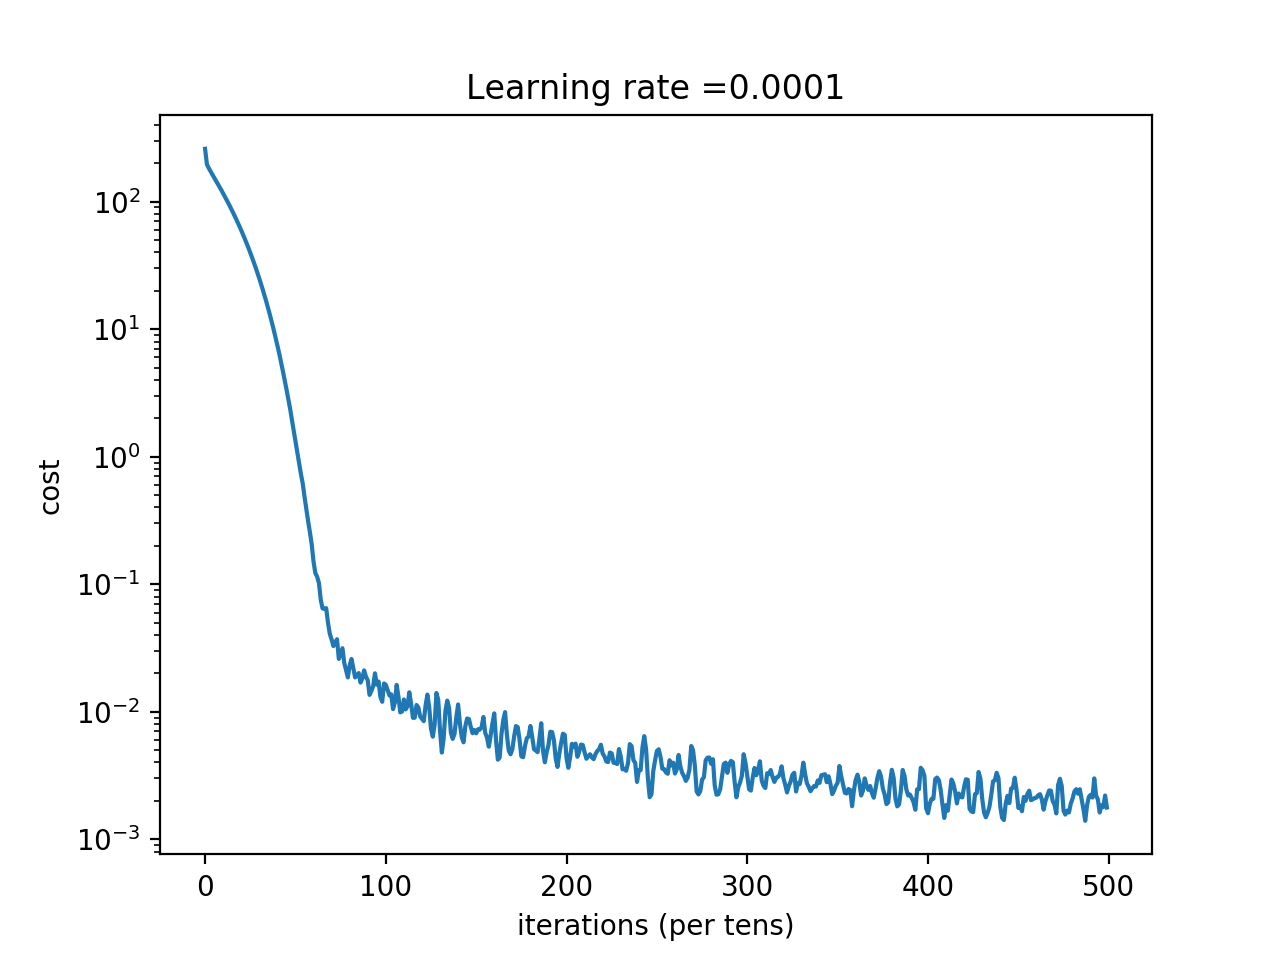
\includegraphics[scale=.75]{figures/cost_vs_epoch_m_3000_minibatch=50.png}
\caption{Cost versus epoch on the training data for problem instance with a possible maximum 
bandwidth of 20 Hz, 3000 examples, a learning rate of 0.0001, and a minibatch size of 50.}
\label{f-example_cost_vs_epoch}
\end{figure}

\paragraph{Work to be completed by the end of the project.} 
The success of the current iteration of the neural network is a promising start, but should be improved upon. 
Most importantly, our current results indicate that there may be a variance problem with our current iteration
of the model. The majority of the time spent until the end of the project will be to experiment with the number of 
layers, the number of nodes per layer, the optimizer selection, the type of regularization used (if 
needed), and the minibatch size. In addition, other types of neural network architectures will be 
considered, such as convolutional neural networks, if they produce better results.

Lastly, a significant portion of time will be spent on communicating my findings via both the poster
presentation and in the final project report.


\newpage
\bibliography{template}

\end{document}